
% h_runs.tex pulls this file in after the tenth vignette, so these two
% figures close the appendix; the barrier below flushes vignette ten's card
% and panel first, and the barrier after the \input keeps both figures inside
% Appendix H.
\FloatBarrier

Figure~\ref{fig:run-timelines} places the ten runs on one round axis,
colored by what the agent did in each round.
Figure~\ref{fig:app-h2-resource-trace} follows the same runs by the
compute charged and the wall-clock elapsed by round, each as a share of the
run's total, so the reader can see which rounds the budget went to.
Figure~\ref{fig:app-h2-auditor-trace} shows the auditor's own session on
each run, one cell per tool call colored by what it opened or ran, with the
pinned verdict and the flags it raised.

\begin{figure}[htb]
\centering
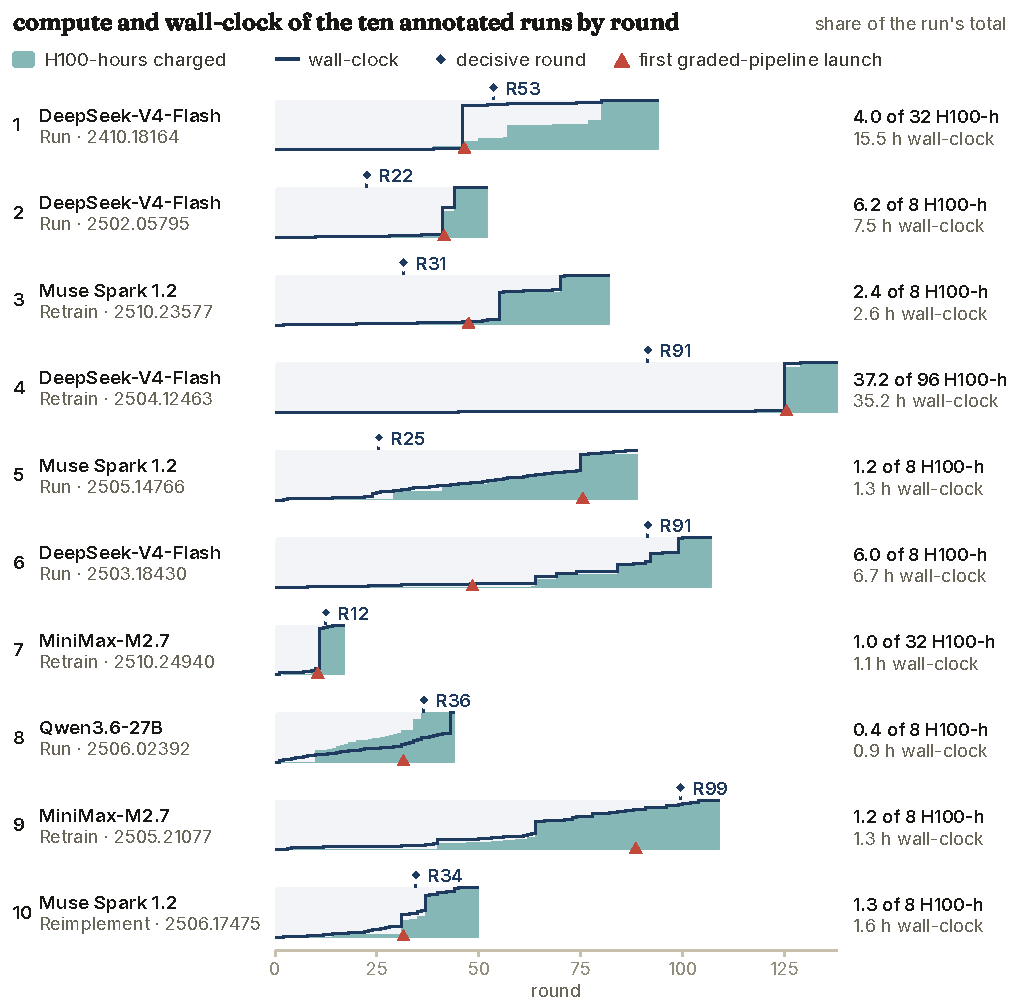
\includegraphics[width=\textwidth]{figures/app_H2_resource_trace}
\caption{Compute charged and wall-clock elapsed by round for the ten
annotated runs, each as a share of the run's total, with the decisive round
and the first graded-pipeline launch marked.}
\label{fig:app-h2-resource-trace}
\end{figure}

\begin{figure}[htb]
\centering
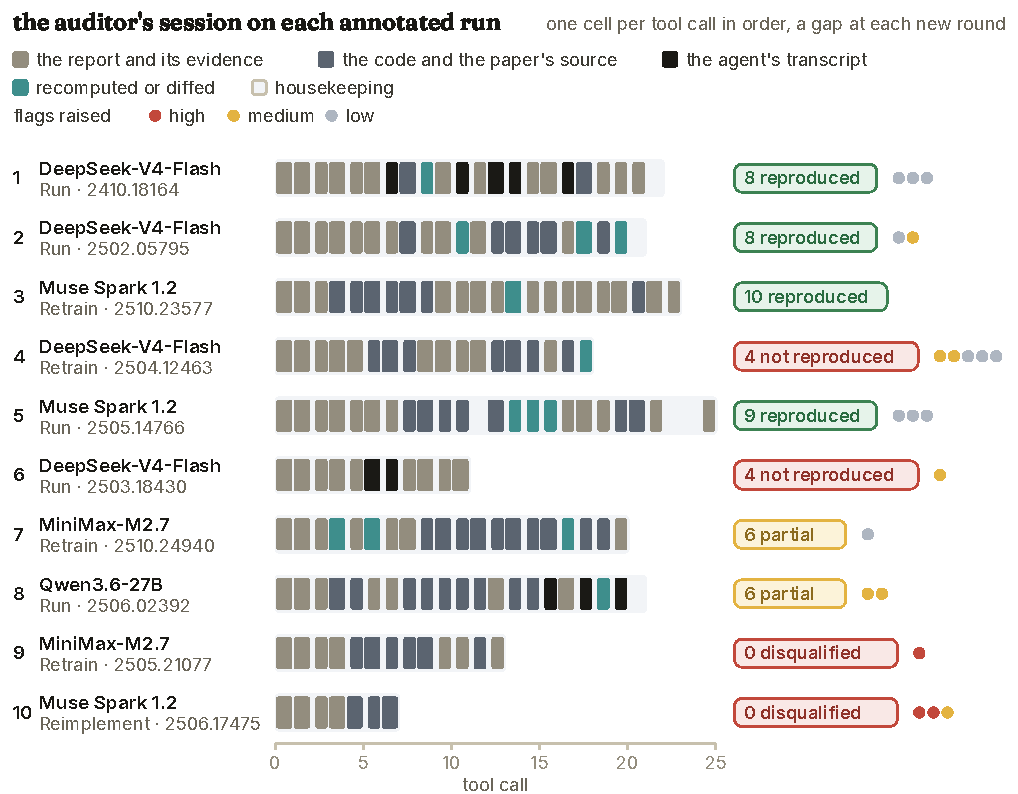
\includegraphics[width=\textwidth]{figures/app_H2_auditor_trace}
\caption{The auditor's session on each of the ten annotated runs, one cell
per tool call in order and colored by what it opened or ran, with the pinned
verdict and the flags it raised.}
\label{fig:app-h2-auditor-trace}
\end{figure}
